\documentclass[10pt,workingdraft]{usetex-v1}
%\documentclass[10pt,workingdraft]{usetex-v1}

\usepackage{todonotes}
\usepackage{epsfig}
\usepackage{url}
\usepackage{times}
%\usepackage{subfigure}
\usepackage{tabularx}
%\usepackage{scalefnt}
%\usepackage{endnotes}
%\usepackage{footnote}
%\usepackage{multirow}
%\usepackage{amsmath}
%\usepackage{amssymb}
%\usepackage{booktabs}
%\usepackage{listings}
\usepackage{vmargin}
\usepackage{cite}
\usepackage{alltt}
%\usepackage{psfrag}
%\usepackage{boxedminipage}
\usepackage{colortbl}
\usepackage{xspace}
%\usepackage{program}


%\numberwithin{equation}{section}
% space b/t list \item's
\newcommand{\smallitemsep}      {\setlength{\itemsep}{-0.5ex}}
%\newcommand{\smallitemsep}     {}

\newcommand{\stt}[1]            {\texttt{\small #1}}

% space b/t captions and their floats
\newcommand{\captionsep}        {\vspace{-1.00em}}
\newcommand{\tabcaptionsep}     {\vspace{-0.50em}}
%\newcommand{\captionsep}       {}
% size of caption font
%\newcommand{\captionfont}      \tiny
\newcommand{\captionfont}       \itshape
\newcommand{\capfont}           \small
%\newcommand{\capfont}          {}

\newcommand{\etal}{\emph{et al.}}

% make tables narrower in width so they fit better in twocolumn formats
\addtolength{\tabcolsep}{-0.5\tabcolsep}
% less space between rows of tables
\renewcommand{\arraystretch}{0.95}
%% space between columns in twocolumn mode
%\addtolength{\columnsep}{-0.1\columnsep}

\newenvironment{consistifyoff}[0]{}      {}

\newenvironment{ezbox}[1]%
{
 \footnotesize
 \begin{center}
 \begin{boxedminipage}[t]{#1}
 \begin{alltt}
}
{
 \end{alltt}
 \end{boxedminipage}
 \end{center}
}

\newenvironment{smalltt}%
{
\vspace{-0.5em}
\footnotesize
\begin{alltt}
}
{
\end{alltt}
\vspace{-0.5em}
}

%\lstset{language=C, basicstyle=\ttfamily\small}
\hyphenation{vnode}

% redefine \url font to normal font
\def\UrlFont{\sl\footnotesize}

\begin{document}

\title{Saving Energy using Green Multi-Disk Driver}

\author{
    \authname{Ming Chen, Rajesh Aavuty, Zhichao Li, and Erez Zadok}
    \authaddr{\{mchen, raavuty, zhicli, ezk\}@cs.stonybrook.edu}
    \authaddr{Department of Computer Science, Stony Brook University}
}

\setpapersize{USletter}
% % \setmarginsrb{leftmargin}{topmargin}{rightmargin}{bottommargin}%
% %    {headheight}{headsep}{footheight}{footskip}
\setmarginsrb{25mm}{25mm}{25mm}{15mm}{0mm}{0mm}{10mm}{10mm}

\pagestyle{plain}

%\newcommand{\stt}[1]                    {\texttt{\small #1}}
%\def\gtilda{\kern -.15em\lower .7ex\hbox{\~{}}\kern .04em}

%%%%%%%%%%%%%%%%%%%%%%%%%%%%%%%%%%%%%%%%%%%%%%%%%%%%%%%%%%%%%%%%%%%%%%%%%%%%%%
%%% SQUEEZE SOME SPACES
%\addtolength{\parskip}{4.5\parskip}
%\setlength{\partopsep}{0mm}
%\setlength{\topsep}{0mm}
%\addtolength{\baselineskip}{-0.03\baselineskip}
%\setlength{\parskip}{-0.5ex}
%\renewcommand{\baselinestretch}{0.9}
%\addtolength{\tabcolsep}{-0.5\tabcolsep}
%\setlength{\topsep}{-2.0ex}
%
%% make tables narrower in width so they fit better in twocolumn formats
%\addtolength{\tabcolsep}{-0.4\tabcolsep}
%% less space between rows of tables
%\renewcommand{\arraystretch}{0.95}
%% allow up to 4 floats at top of page (default=2)
\setcounter{topnumber}{4}
\setcounter{dbltopnumber}{8}	% for double-floats
%% allow up to 2 floats at bottom of page (default=1)
\setcounter{bottomnumber}{2}
%% allow up to 8 floats total per page (default=3)
\setcounter{totalnumber}{8}

% %% less space above/below floats that are at top/bottom of pages
\addtolength{\floatsep}{-0.5\floatsep}
\addtolength{\dblfloatsep}{-0.5\dblfloatsep}
% %% less space above/below "h" floats that are in the middle of text
\addtolength{\intextsep}{-0.5\intextsep}
\addtolength{\textfloatsep}{-0.5\textfloatsep}
\addtolength{\dbltextfloatsep}{-0.5\dbltextfloatsep}
% smaller space around captions
\addtolength{\abovecaptionskip}{-0.75\abovecaptionskip}

%% Control floats
\renewcommand{\topfraction}{1.0} % max percentage a float can take at top
\renewcommand{\bottomfraction}{1.0} % max percentage float can take at bottom
\renewcommand{\textfraction}{0.01} % min percentage text can take on page
%\renewcommand{\textfraction}{0.5} % min percentage text can take on page
\renewcommand{\floatpagefraction}{0.99} % min fraction of float page used
\renewcommand{\dblfloatpagefraction}{0.99} % min fraction of float page used

%% space between columns in twocolumn mode
%\addtolength{\columnsep}{-0.1\columnsep}
%% width of text on a page
%\addtolength{\textwidth}{0.01\textwidth}

%%%%%%%%%%%%%%%%%%%%%%%%%%%%%%%%%%%%%%%%%%%%%%%%%%%%%%%%%%%%%%%%%%%%%%%%%%%%%%

%\tableofcontents
\maketitle

\begin{abstract}

% dummy entry to force emacs not to indent abstract text
\vspace{0mm}

\todo[color=blue!40,inline]{Zhichao: we have updated the project plan
for the class because of the limited time. Therefore, please make sure 
the abstract matches what will be presented in the report. }

Storage subsystems in servers are slower than other subsystems despite
the fact that they contribute to a large portion of the total power
consumption. Hybrid disks, which integrate different characteristics
of various kinds of disks (e.g., SATA, SAS, SSD) in speed, capacity,
price, and power consumption, is a promising solution to the problem.
While researches on hybrid disk have reported significant performance
boost over traditional magnetic disks, their energy usage is less
studied.  In this project, we consider energy efficiency of storage
systems as important as performance and capacity.  Our goal is to
provide a multi-disk system that consists of different disks, provides
a capacity equal to the sum of all disks, operates at a speed near the
fastest disk, but consume less energy than the sum of all disks when
they operate individually.

To achieve energy efficiency as well as good performance, our
multi-disk system tries to map more frequently accessed blocks (i.e.,
hot data) to energy-efficient, fast, but small disks such as SSD.
Conversely, cold data goes to inefficient, slow, but large disks such
as SATA.  This exploits spatial locality of data and has similar
effect in hybrid model where SSD is used as cache disk.  Meanwhile,
temporal locality of data is also be exploited to group blocks that
are likely to be accessed simultaneously.  Instead of scattering
blocks among several disks, we try to map them to a single disk.  The
combination of spatial and temporal locality allows I/O be served
using fewer disks and other disks can spin down to save energy.  To
identify hot data and block groups, workload-specific traces are
analyzed offline. Online statistics will also be gathered and used by
heuristic algorithm for adaption to hot data and block groups as they
evolve over time. We are also exploring naive direct IO map without
any knowledge of the workloads as baseline approach. 

\end{abstract}

%%%%%%%%%%%%%%%%%%%%%%%%%%%%%%%%%%%%%%%%%%%%%%%%%%%%%%%%%%%%%%%%%%%%%%%%%%%%%%
%% For Emacs:
% Local variables:
% fill-column: 70
% End:
%%%%%%%%%%%%%%%%%%%%%%%%%%%%%%%%%%%%%%%%%%%%%%%%%%%%%%%%%%%%%%%%%%%%%%%%%%%%%%
%% For Vim:
% vim:textwidth=70
%%%%%%%%%%%%%%%%%%%%%%%%%%%%%%%%%%%%%%%%%%%%%%%%%%%%%%%%%%%%%%%%%%%%%%%%%%%%%%
% LocalWords:  

\section{Introduction}
\label{intro}


Increasing IT demand has seen 6$\times$ growth of server and
69$\times$ growth of storage during the last decade
\cite{ibm_green_beyond}. Data centers energy use is doubling every 5
years, whereas the global electricity prices are increasing 10--25\%
per year. The energy efficiency of computer systems becomes
increasingly interesting to academic and industrial communities.
Studies show that storage systems are responsible not only for the
system performance bottleneck but also for up to 40\% of the power
consumption\cite{storage_40}. This is largely due to the inherent
drawback of traditional hard disks (HDD), which consist of physical
moving parts. They consume a lot of power to keep disk platters
spinning at a high speed and they are slow as disk heads have to move
to the right position before serving random I/O.

Thanks to the development of solid state drive (SSD) technology, many
of the problems related to performance and energy efficiency are
alleviated. However, despite having the above advantages, SSDs are
not widely adopted in the server storage stack due to their high
capital cost per byte. To overcome this limit, hybrid disks are
proposed. Hybrid disks achieve better trade-off between performance
and capacity by organizing different disks in the manner conformant to
the storage hierarchy. 

The most common type of hybrid disks \cite{Bisson07ahybrid} tries to
reap the benefits of SSDs by having a small flash memory on each hard
disk and using this flash memory as \mbox{non-volatile} cache for the
hard disk. A host can use this \mbox{non-volatile} cache to achieve
faster random reads since it is fast and takes constant time to access
any block in the SSD cache. Although this type of hybrid disk improves
performance over traditional disks, the improvement was modest due to
the relatively small size of \mbox{non-volatile} cache on each disk.
It is also difficult to balance the cache load among disks because the
SSD caches are separated among disks. For example, if a workload
accesses one disk more frequently than others, then this could result
in frequent cache misses on that particular disk, while the caches on
other disks are under-utilized. 

To enable servers to benefit more from the power efficiency and high
performance of solid state media, we used a single but relatively
large SSD to store hot data. We store other data in other less
efficient disks. The SSD is referred as cache disk, and all other
disks are referred as secondary disks. This approach achieves a good
cache hit ratio because of the large size of the cache. Thanks to data
locality, it makes the SSD capable of serving the majority of the disk
accesses as we can see in previous systems with large SSD cache
\cite{Debnath_SkimpyStash, Debnath_Bloomflash,
flashcache_experiments}. Therefore, other disks are idle for longer
periods of time and thus can be powered down to save energy. 

%The difference between the above two types of hybrid disks seems to be
%not clear if we consider the virtualization of disk such as Linux
%Logical Volume Management (LVM). By grouping all hard disks to form a
%single virtual disk, the cache on all these hard disks can be gathered
%together which becomes equivalent to the large SSD we are using. This
%workaround alleviates the load balance problem. However, it is less
%helpful in saving energy because the virtualization of multi-disk is
%not aware of energy efficiency. If there are non-adjacent blocks that
%are often simultaneously accessed, we can perform data grouping and
%store them onto one physical disk so that only this disk has to spin
%up when they are accessed. In this case, the optimization cannot be
%achieved if the LVM virtualization approach is employed. 

To exploit spatial and temporal data locality to the largest extent,
we collected workload-specific traces and are trying to find hot data
and block groups of working sets. For hot data, we simply find blocks
that are most frequently accessed. We realize that hot data changed
over time. However, this offline study is still helpful because some
data is inherently hot. (e.g., file-system metadata and latest data).
Moreover, because our analysis is workload specific, it is likely the
same I/O pattern repeats in the same or similar workload. We also try
to keep hot data in the cache online using an LRU algorithm. To
identify block groups, we use methods in Avani's work
\cite{Wildani_grouping} to map blocks that are simultaneously accessed
to same physical disk so that fewer disks are required to power up.
Additionally, data grouping has a benefit of isolating faults because
blocks of working sets are more concentrated and physical failure of
one disk affects fewer working sets \cite{Sivathanu_dgraid,
Wildani_grouping}. 

We use the Linux Device Mapper (DM) framework and implement our hybrid
model as a Device Mapper target. This provides modularity and
transparency as it enables us to create virtual disks without exposing
the details of underlying physical disks. To be reliable, we use
SSD-aware algorithms in our implementation to alleviate the short life
time problem of SSD. We also periodically flush metadata onto disks to
prevent machine failure from destroying our block mapping. By
leveraging the strengths of different kinds of disks, our virtual disk
can better trade-off among power consumption, I/O performance, and
storage capacity.

The rest of the paper is organized as follows. Section
\ref{sec:design} describes our design and implementation. Section
\ref{sec:trace} presents block trace analysis. We evaluate the energy
efficiency and I/O performance of our system in Section
\ref{sec:eval}. We analyze related work in Section \ref{sec:related}
and conclude our work in Section \ref{sec:conc}.

%%%%%%%%%%%%%%%%%%%%%%%%%%%%%%%%%%%%%%%%%%%%%%%%%%%%%%%%%%%%%%%%%%%%%%%%%%%%%%
%% For Emacs:
% Local variables:
% fill-column: 70
% End:
%%%%%%%%%%%%%%%%%%%%%%%%%%%%%%%%%%%%%%%%%%%%%%%%%%%%%%%%%%%%%%%%%%%%%%%%%%%%%%
%% For Vim:
% vim:textwidth=70
%%%%%%%%%%%%%%%%%%%%%%%%%%%%%%%%%%%%%%%%%%%%%%%%%%%%%%%%%%%%%%%%%%%%%%%%%%%%%%
% LocalWords:  

%\input{bg}
\section{Design}
\label{Design}

\begin{figure}[ht]
\begin{centering}
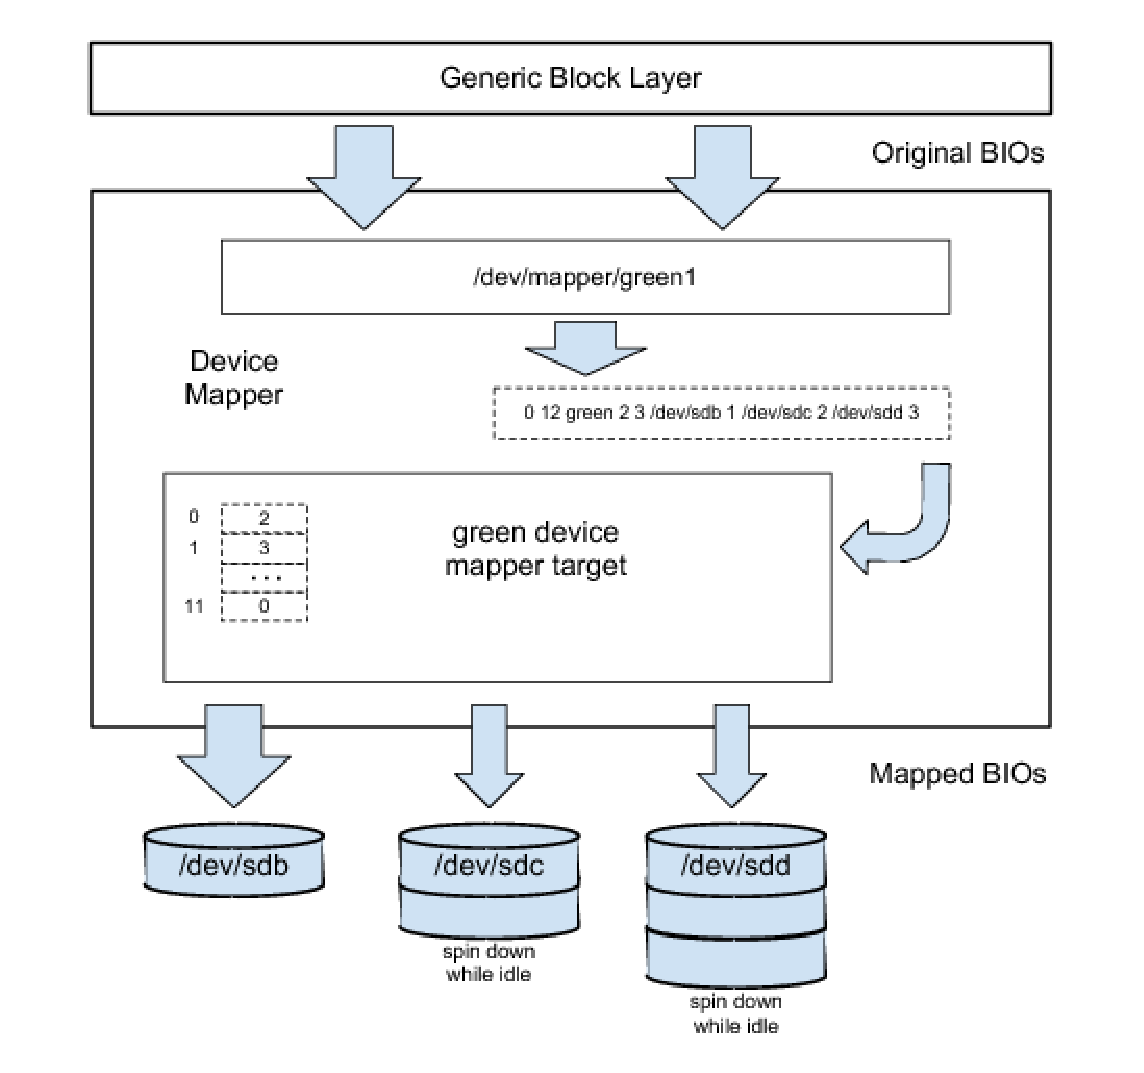
\epsfig{file=figures/dm.eps,width=1.00\linewidth}
\caption{Linux Device Mapper and Green Device Mapper Target.
/dev/mapper/green1 is a virtual block device. The two dashed boxes are
mapping tables. The first one is used by Device Mapper to delegate
mapping to target; the second one is used internally by the green
target.}
\label{fig:dm}
\end{centering}
\end{figure}

We present the design of our green multi-disk driver as a Linux Device
Mapper target. Linux Device Mapper, as depicted in Figure
\ref{fig:dm}, is a generic framework to map one block device onto
another. It works by processing data passed in from a virtual block
device, that it itself provides, and then passing the resultant data
on to another block device. The advantage of Device Mapper is that it
can provide virtual devices to user programs and kernel modules above
block level without exposing details of underlying devices. Thanks to
this transparency, the underlying devices can be of different size and
type (can in turn be virtual or physical) and the mapping can be
performed in different ways. Device mapper is essentially a
middle-ware sitting between the Generic Block Layer and block devices.
It receives BIOs, which is a kernel structure describe I/O requests,
from Generic Block Layer, then redirect them to other block devices by
modifying the target device and target sector. 

Device Mapper itself does not perform the redirection. It delegates
this operation to Device Mapper targets, which are registered kernel
modules performing certain kinds of mapping. This delegation is
specified in a mapping table, which contains the type of responsible
Device Mapper target for certain regions of block devices. In Figure
\ref{fig:dm}, all I/O request to sectors [0, 0+12) of virtual device
"/dev/mapping/green1" will be handled by a target named green; all
parameters after "green" are passed to the green target. A mapping
target which contains functions to construct/destruct mapped devices,
map I/O requests, merge adjacent I/O requests, report and control
device status.

\subsection{Design Goals}
The design goal of our green multi-disk driver is driven by the
following guiding principles: 

\begin{itemize}
\item \textbf{Save energy by allowing disks to spin/power down}. Be
energy efficiency is one of the most important feature our green
multi-disk driver is pursuing. The SSD cache benefits both I/O
performance and energy efficiency benefit. In this study, we are more
concerned of the latter and there is tradeoff between the two. 

\item \textbf{Use SSD aware data structures and algorithms}. While SSD
provides better I/O performance and energy efficency, it has its own
constraints including limited eraze-write cycles and inefficient
random writes. This principle guides our design to avoid these
constraints and extract maximum benefit out of SSD.

\item \textbf{Provide stable and robust storage}. Because our green
target provides customized data mapping and block grouping, it is
critical to always perform correct translation between virtual and
physical blocks. It should not lose data in case of power failure or
other hazardous conditions.
\end{itemize}

\subsection{Disk Management}

Device Mapper targets maintain mapping of sectors between virtual and
physical disks. The straightforward method is to maintain a
sector-wise mapping table. However, it is prohibitive because its size
is too large to fit in memory. For example, the size of sector-wise
mapping table of a 1TB disk (512-byte sectors) is as large as 8GB with
4-bytes table entries. Store the mapping table on disk (even on SSD)
is not an option because it is too slow to incur extra I/O. A solution
is to divide disks into larger unit. Here, we adopt the LVM term
extent, which is the unit of disk managed by LVM, typically 4MB. Then
the mapping becomes extent-wise and its size diminishes to 1MB in the
above example. 

In the green target, multiple physical disks are mapped as a single
virtual disk. They will be kept in the order of energy efficiency,
i.e., the most energy-efficient goes first and so on. In Figure
\ref{fig:dm}, '/dev/sdb' is the most energy-efficient one but with
smallest capacity, i.e., SSD; '/dev/sdc' and '/dev/sdd' follow
decreasingly in energy-efficiency and increasingly in capacity. This
makes the addressing of physical sectors easy. An extent index and an
offset within extent suffice. We have noticed the case that one IO
request on logically sequential blocks might be mapped to multiple IO
requests on physically non-sequential blocks. Therefore, the
translation is performed per extent instead of per request. However,
extent is of big size, so it is unlikely that the extent by extent
translation is a performance bottleneck. It is not a problem also
because the Device Mapper framework provides interface to merge
adjacent I/O requests. 

The exact size of extent is an important factor as it affects not only
memory consumption but also granularity of mapping. A large size of
extent has the following impacts: 

\begin{itemize} 
\item \textbf{Smaller mapping table}. As already discussed, the
adoption of extent makes the mapping table becomes extent-wise and its
size is reduced. 

\item \textbf{More aggresive prefetch}. As energy-efficient disk such
as SSD have similar effect as disk cache. When a large extent of data
is move onto SSD, it can be consider as an aggresive prefetch. 

\item \textbf{Coarse-grain data migration among disks and more
sequential I/O}. Because the major lantency of magnetic disk is seek
time, a larger sequential access will not significantly slow down the
IO. Moreover, with large size of migration unit, there are fewer IO
because adjacent sectors can be grouped. This is benefical to the life
time of SSD as well considering its limited write-erase cycles.

\item \textbf{High overhead}. Since each extent can represent several
sectors, depends on the workload IO, more sectors IO can be wasteful
and only adds overhead to the overall system. 

\end{itemize}

Different workloads might also favor different extent sizes
considering file sizes and I/O frequency. Therefore, we make it a
configurable parameter to the green target so that different
trade-offs can be made by configuration. 

\subsection{Mapping Table}

There are two mapping tables. One is actually a configuration file
used by the Device Mapper framework; the other contains extent-wise
mapping information used internally by our green target. We are
talking about the second one in following discussion. 

The straightforward structure of the mapping table is an array of the
size of total extent number. The mapping table is maintained in memory
and can be cached, so its lookup is fast. Besides mapping information,
the table also contains other fields including flags, timestamp of the
latest access and number of total access (possibly distinguished
between read and write). Flags are used to record states of extents,
which may include for example 1) whether the extent is accessed or
not; 2) whether the extent is under migration or not; and 3) whether
the extent is updated or not when it is under migration. Timestamp of
the latest access and number of total access are used to predict hot
extent. Their use will be discussed in next section. 

The mapping table need be saved to disk on power off as metadata. To
be fail-safe, it has a replicate in every physical disk. The in-memory
version and on-disk version of mapping table can be slightly
different, since it is not necessary to save online information such
as timestamp of latest access. Moreover, to be robust in case of
hazardous situation such as power failure, the mapping table is
flushed onto disk periodically. To prevent this periodical background
job from interrupting other disk, it only save the table on the cache
disk. Table on other disks are only updated on request or when the
system is being shutting down.

%-----------------------------------------------------------------------------

\subsection{Extent Migration}
There are two kind of extent movements. The first is the movement
between the SSD cache disk and secondary disks. The second is the
movement between secondary disks. The first kind of movement is
actually cache loading and eviction. It is neccessary for ensuring
that we always maintain hot extents on cache disk. LRU algorithm is
used in this case. The second movement, which is extent migration,
happens when there is a need to keep all extents of a working set on a
single physical disk. 

\subsection{Trace Study}

Trace analysis plays a crucial role in identifying hot data blocks
across different disks. The idea is to move hot blocks to cache disk
and serve most of the requests from the energy-efficient cache disk
and hence spin/power down other secondary disks for long periods of
time to achieve good power savings and increased performance. I/O
block traces can be used both in offline mode and online mode. In
offline mode, first we collect traces for a particular workload and
later analyze these traces to tweak important parameters. For example,
a good value for parameters like extent size and migration threshold
can be decided by studying the traces for a workload. In online mode,
we use I/O block traces to dynamically identify hot blocks across
different disks. First, the traces are collected for a particular
workload and analyze these traces to identify any patterns in the I/O
accesses. If we can find a particular trend in workloads (which is
more likely for server workloads), we use trace analysis to
dynamically identify hot working sets. Workloads for video servers and
file servers are more likely to exhibit good data locality property as
only a fraction of files are popular at a particular instant and the
distribution of popular files on disks change dynamically. Also We
expect IOs of these workloads to be largely sequential in nature.
Sequential workloads are more suitable for this approach 

Right now, we use I/O traces for analysis and tweaking parameters. I/O
traces can also be used in online mode to predict the hot blocks. This
approach is another option and we may implement this if time permits.
Also, to verify the correctness and working of our concept, We will
replay the traces with and without green Multi-disk target and compare
the power consumption and I/O performance. 

We ran the workloads for a relatively long periods (for a few hours).
We used blktrace tool to collect traces. Block traces would contain
information like disk major and minor number, disk offset, number of
blocks accessed , Read/Write information  and timestamp for every I/O
sent to disk. We us the pertinent I/O information from the traces to
identify workload characteristics.

\begin{figure}[ht]
\begin{centering}
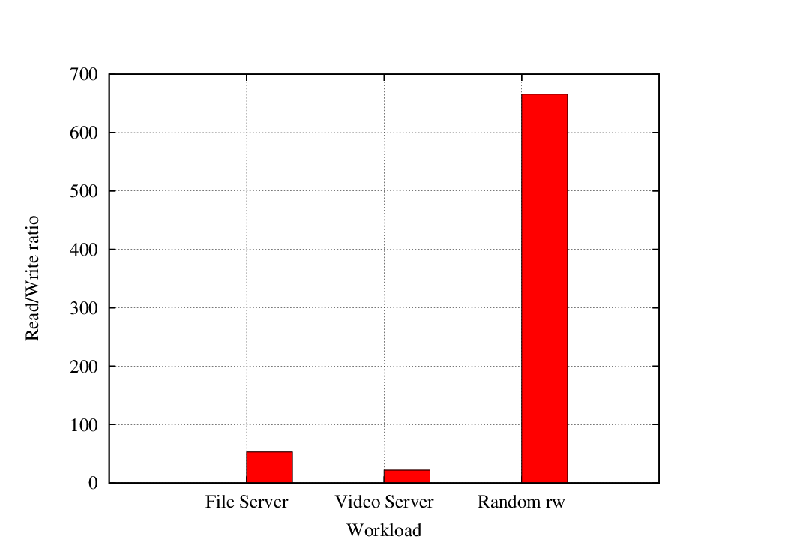
\epsfig{file=figures/rw.eps,width=1.00\linewidth}
\caption{Read/Write Ratio from Analysis of Workload Traces.}
\label{fig:rw}
\end{centering}
\end{figure}

In Figure \ref{fig:rw}, we present the graphs for Read/Write ratio for
three different workloads, namely random read/write, videoserver and
fileserver workloads. All these workloads were generated using
filebench and each workload was run for 2 hours. We used three
different physical disks with different power consumption and
performance characteristics to run these workloads.   

%%%%%%%%%%%%%%%%%%%%%%%%%%%%%%%%%%%%%%%%%%%%%%%%%%%%%%%%%%%%%%%%%%%%%%%%%%%%%%
%% For Emacs:
% Local variables:
% fill-column: 70
% End:
%%%%%%%%%%%%%%%%%%%%%%%%%%%%%%%%%%%%%%%%%%%%%%%%%%%%%%%%%%%%%%%%%%%%%%%%%%%%%%
%% For Vim:
% vim:textwidth=70
%%%%%%%%%%%%%%%%%%%%%%%%%%%%%%%%%%%%%%%%%%%%%%%%%%%%%%%%%%%%%%%%%%%%%%%%%%%%%%
% LocalWords:  

\section{Trace Study}
\label{sec:trace}

Traces are used to collect information about the system workloads.
Traces can be collected at different layers in storage stack. Block
traces would contain information about disk offset, number of blocks
accessed, Read/Write information and timestamp for every accessed I/O.
This information can be used to characterize the workloads and
identify I/O access patterns.  Trace analysis plays a crucial role in
identifying hot data blocks across different disks.The idea is to move
hot blocks to primary disk and serve most of the requests from most
energy efficient disk. Hence other disks can be spun/powered down for
long periods of time to achieve good power savings and increased
performance. A simple approach like counting the number of times a
particular block is accessed can be used to find the hotness of disk
blocks. Apart from this, I/O block traces can be used for variety of
other purposes.  For example, block trace analysis can be used to
tweak the design parameters like extent size and migration threshold.

Workloads which exhibit good data locality properties are most
suitable for this project. Workloads such as video server and file
server are likely to exhibit this property. The distribution of
popular files on disks may change dynamically but at any particular
instant, only a fraction of files the disk are popular in the case of
above workloads.  A workload which is completely random I/O access
patterns would not benefit this approach as it would result in
frequent data migration between primary disks and secondary disks.
 
Currently, we use I/O traces for analysis and tweaking parameters. I/O
traces can also be used in offline mode to predict the hot blocks.
This approach is another option and we may implement this if time
permits. Also, to verify the correctness and working of our concept,
we replay the traces with and without green Multi-disk target and
compare the power consumption and I/O performance. 

\begin{figure}[ht]
\begin{centering}
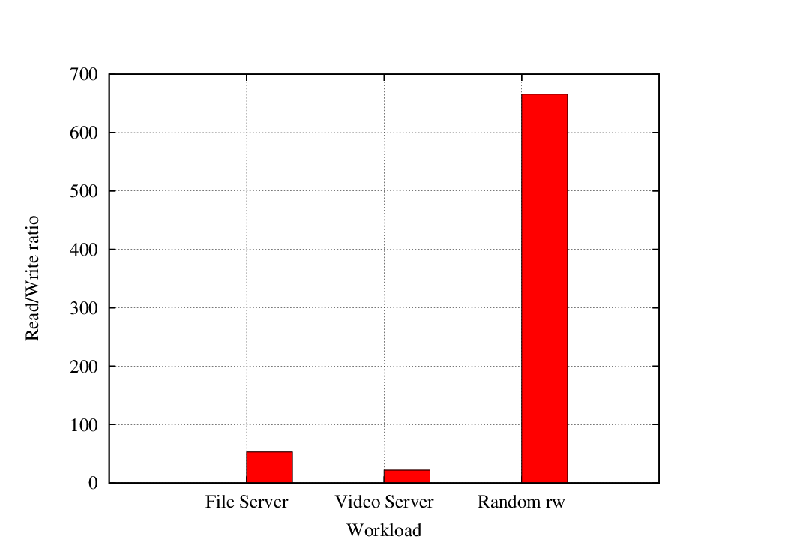
\epsfig{file=figures/rw.eps,width=1.00\linewidth}
\caption{Read/write ratio of video server, file server and random
  workloads.}
\label{fig:rwratio}
\end{centering}
\end{figure}

\begin{figure}[ht]
\begin{centering}
\epsfig{file=figures/randomrw_io_freq.eps,width=1.00\linewidth}
\caption{I/O size of the random workload.}
\label{fig:randomiosize}
\end{centering}
\end{figure}

I/O block traces have been collected for variety of workloads like
video server, file server and random workloads. The workloads were run
for a relatively long periods (for a few hours). Below, we present the
results for some preliminary analysis on the traces. Figure
\ref{fig:rwratio} shows Read/Write ratios for the above three
workloads.  We have collected the number of times a particular I/O
size was issued for the above three workloads. Figure
\ref{fig:randomiosize}, which shows the I/O size of the random
workloads, is one of them. All these workloads were generated using
Filebench and each workload runs for 2 hours. We used three different
physical disks with different power consumption and performance
characteristics to run these workloads. 

%%%%%%%%%%%%%%%%%%%%%%%%%%%%%%%%%%%%%%%%%%%%%%%%%%%%%%%%%%%%%%%%%%%%%%%%%%%%%%
%% For Emacs:
% Local variables:
% fill-column: 70
% End:
%%%%%%%%%%%%%%%%%%%%%%%%%%%%%%%%%%%%%%%%%%%%%%%%%%%%%%%%%%%%%%%%%%%%%%%%%%%%%%
%% For Vim:
% vim:textwidth=70
%%%%%%%%%%%%%%%%%%%%%%%%%%%%%%%%%%%%%%%%%%%%%%%%%%%%%%%%%%%%%%%%%%%%%%%%%%%%%%
% LocalWords:  SMR HDDs drive's SMRs

\section{Evaluation}
\label{eval}

We have finished the code. But it is still being tested. We are going
to perform experiments to evaluate our system in the near future.

%%%%%%%%%%%%%%%%%%%%%%%%%%%%%%%%%%%%%%%%%%%%%%%%%%%%%%%%%%%%%%%%%%%%%%%%%%%%%%
%% For Emacs:
% Local variables:
% fill-column: 70
% End:
%%%%%%%%%%%%%%%%%%%%%%%%%%%%%%%%%%%%%%%%%%%%%%%%%%%%%%%%%%%%%%%%%%%%%%%%%%%%%%
%% For Vim:
% vim:textwidth=70
%%%%%%%%%%%%%%%%%%%%%%%%%%%%%%%%%%%%%%%%%%%%%%%%%%%%%%%%%%%%%%%%%%%%%%%%%%%%%%
% LocalWords:  

\section{Related Work} 
\label{sec:related} 

Our study provides a multi-disk (hybrid) system in the purpose of
saving energy. To achieve that, we use energy-efficient disk as cache
and perform data migration and grouping using information obtained
from traces study. We discuss related work that covers the following
aspects: save energy, hybrid disk, data grouping and workload trace
study.

\textbf{Save Energy}. Energy efficiency of storage systems is an
interesting problem that is being actively researched. Sehgal et al.
\cite{fast10fsgreen} studied the power consumption of servers when
different workloads are running. Kothiyal et al.
\cite{systor09greencomp} presented empirical analysis of how lossless
compression influences power consumption of servers. Li et al.
\cite{fast12emc-energy} presented the first study of power consumption
of really running enterprise-scale backup systems. A category of
methods to save energy is using data replication to decrease either
disk head movement \cite{huangfs2, pred_data_grouping} or the number
of active disks being used \cite{Weddle07paraid}. 

\textbf{Hybrid disk}. There are various studies of hybrid disk,
wherein SSDs were used as cache disks \cite{Bisson07ahybrid,
Debnath_SkimpyStash, Debnath_Bloomflash, flashcache_experiments}.
Among them, few of them was really focusing on the energy efficiency
aspect of hybrid disk\cite{Bisson07ahybrid}. Although Zhu et al.
\cite{Zhu04reducingenergy} was also studying power aware cache, their
cache was in volatile RAM instead of non-volatile disk. Carrera et al.
\cite{slow_fast} presented a hybrid storage system that combines low
and high speed disks to save energy.

\textbf{Data grouping}. Wildani et al. \cite{Wildani_grouping}
presented data grouping of working set, however, their work only
contained analysis of offline traces. It was not implemented or
experimented on real system. The Energy-Efficient File System (EEFS)
groups files with high temporal access locality
\cite{Li06highperformance}. Essary et al. \cite{pred_data_grouping}
also performed predictive data grouping to reduce head movements for
saving energy.  Pinheiro and Bianchini \cite{migration04} used the
fact that regularly only a small subset of data is accessed by a
system, and migrated frequently accessed data to a small number of
active disks, keeping the remaining disks off, which is a kind of data
grouping.

\textbf{Trace study}. Trace extraction is a popular method used by
system researchers to analyze the system behavior. The analysis can be
used to optimize several important features of the system like CPU and
memory utilization, I/O throughput, latency, etc. Several reseachers
have used trace analysis to find correlations between disk block
accesses. Z. Li et al \cite{Li04c-miner} used data mining techniques
to find block correlations. T. Li et al \cite{Li_model} used block
traces to to run-time modeling to estimate the power consumption of
servers. Douglas et al. \cite{Douglis_95} used efficient algorithms
based on machine learning techniques on block traces to spin down
disks and extend battery life in mobile computers. V. Torasov
\cite{fast12t2m} used trace analysis to evaluate performance and
energy efficiency in file system server workloads extensions.


%%%%%%%%%%%%%%%%%%%%%%%%%%%%%%%%%%%%%%%%%%%%%%%%%%%%%%%%%%%%%%%%%%%%%%%%%%%%%%
%% For Emacs:
% Local variables:
% fill-column: 70
% End:
%%%%%%%%%%%%%%%%%%%%%%%%%%%%%%%%%%%%%%%%%%%%%%%%%%%%%%%%%%%%%%%%%%%%%%%%%%%%%%
%% For Vim:
% vim:textwidth=70
%%%%%%%%%%%%%%%%%%%%%%%%%%%%%%%%%%%%%%%%%%%%%%%%%%%%%%%%%%%%%%%%%%%%%%%%%%%%%%
% LocalWords:  SMR HDDs drive's SMRs

\section{Conclusions}
\label{conc}
Not finished.

\paragraph{Future Work} 
%

\begin{itemize}
\item Make the code running correctly. 

\item Replay traces on virtual devices created by our green target;
compare energy consumption of multi-disk of linear mapping and out
green multi-disk.
\end{itemize}

%%%%%%%%%%%%%%%%%%%%%%%%%%%%%%%%%%%%%%%%%%%%%%%%%%%%%%%%%%%%%%%%%%%%%%%%%%%%%%
%% For Emacs:
% Local variables:
% fill-column: 70
% End:
%%%%%%%%%%%%%%%%%%%%%%%%%%%%%%%%%%%%%%%%%%%%%%%%%%%%%%%%%%%%%%%%%%%%%%%%%%%%%%
%% For Vim:
% vim:textwidth=70
%%%%%%%%%%%%%%%%%%%%%%%%%%%%%%%%%%%%%%%%%%%%%%%%%%%%%%%%%%%%%%%%%%%%%%%%%%%%%%
% LocalWords:  

%\paragraph{Acknowledgments}
\label{ack}

1 pgf max.

Optional if you have space.  Cannot ack in anonymous
submissions.

List anyone who helped ideas, review drafts, but isn't a
co-author.

List any funding agency that supported the work (some agencies
require this).

Example:

We thank the EMC/Data Domain performance team for their help.  We also
thank Windsor Hsu, our shepherd Jiri Schindler and our anonymous
reviewers for their helpful feedback.  This work was supported in part
by NSF award CCF-0937854.



%%%%%%%%%%%%%%%%%%%%%%%%%%%%%%%%%%%%%%%%%%%%%%%%%%%%%%%%%%%%%%%%%%%%%%%%%%%%%%
%% For Emacs:
% Local variables:
% fill-column: 70
% End:
%%%%%%%%%%%%%%%%%%%%%%%%%%%%%%%%%%%%%%%%%%%%%%%%%%%%%%%%%%%%%%%%%%%%%%%%%%%%%%
%% For Vim:
% vim:textwidth=70
%%%%%%%%%%%%%%%%%%%%%%%%%%%%%%%%%%%%%%%%%%%%%%%%%%%%%%%%%%%%%%%%%%%%%%%%%%%%%%
% LocalWords:  SMR HDDs drive's SMRs

%\clearpage

% \appendix
% \input{appendix}

\bibliographystyle{plain}
\bibliography{template/master,smr,gos}
%{\footnotesize \bibliography{template/master}}

%\newpage

\end{document}

%%%%%%%%%%%%%%%%%%%%%%%%%%%%%%%%%%%%%%%%%%%%%%%%%%%%%%%%%%%%%%%%%%%%%%%%%%%%%%
%% For Emacs:
% Local variables:
% fill-column: 70
% End:
%%%%%%%%%%%%%%%%%%%%%%%%%%%%%%%%%%%%%%%%%%%%%%%%%%%%%%%%%%%%%%%%%%%%%%%%%%%%%%
%% For vim:
% vim:textwidth=70
%%%%%%%%%%%%%%%%%%%%%%%%%%%%%%%%%%%%%%%%%%%%%%%%%%%%%%%%%%%%%%%%%%%%%%%%%%%%%%
% LocalWords:

% LocalWords:  Ankur Agrawal Benixon Arul Dhas Hospodor Yangwook Kang Rekha UC
% LocalWords:  Pitchumani Sphurti Sortur USletter csrg smr
